\documentclass{article}
\usepackage[margin=.8in]{geometry}
\usepackage{multicol}
\usepackage{blindtext}
\usepackage{graphicx}
\usepackage{pgfplots}
\usepackage{pgfplotstable}
\usepackage{tikz}
\usetikzlibrary{shapes.geometric, arrows}
\usepackage{listings}
\usepackage{array}
\usepackage{amsmath}
\usepackage{tabularx}

\definecolor{testorange}{HTML}{FFAD7A}
\definecolor{clear}{HTML}{E3E9FD}
\definecolor{magenta}{HTML}{C60059}
\definecolor{yellow}{HTML}{f0a000}
\definecolor{cyan}{HTML}{0089A6}
\definecolor{targetblue}{HTML}{1a4d66}

\title{PolyJet Voxel Printing Exploration}

\author{Jack Crane}
\date{\today}

\begin{document}

\noindent
\LARGE\textsl{Printing complex geometry with complex materials}
\vspace*{-.1cm} 

\noindent
\Huge Translating images into Voxel Print-ready slices
\vspace*{.2cm} 

\noindent
\large Jack Crane \textit{jack.crane@slu.edu}

\noindent
\large Saint Louis University Center for Additive Manufacturing \textit{slu.cam@slu.edu}
\normalsize

\vspace{.2in}

\noindent
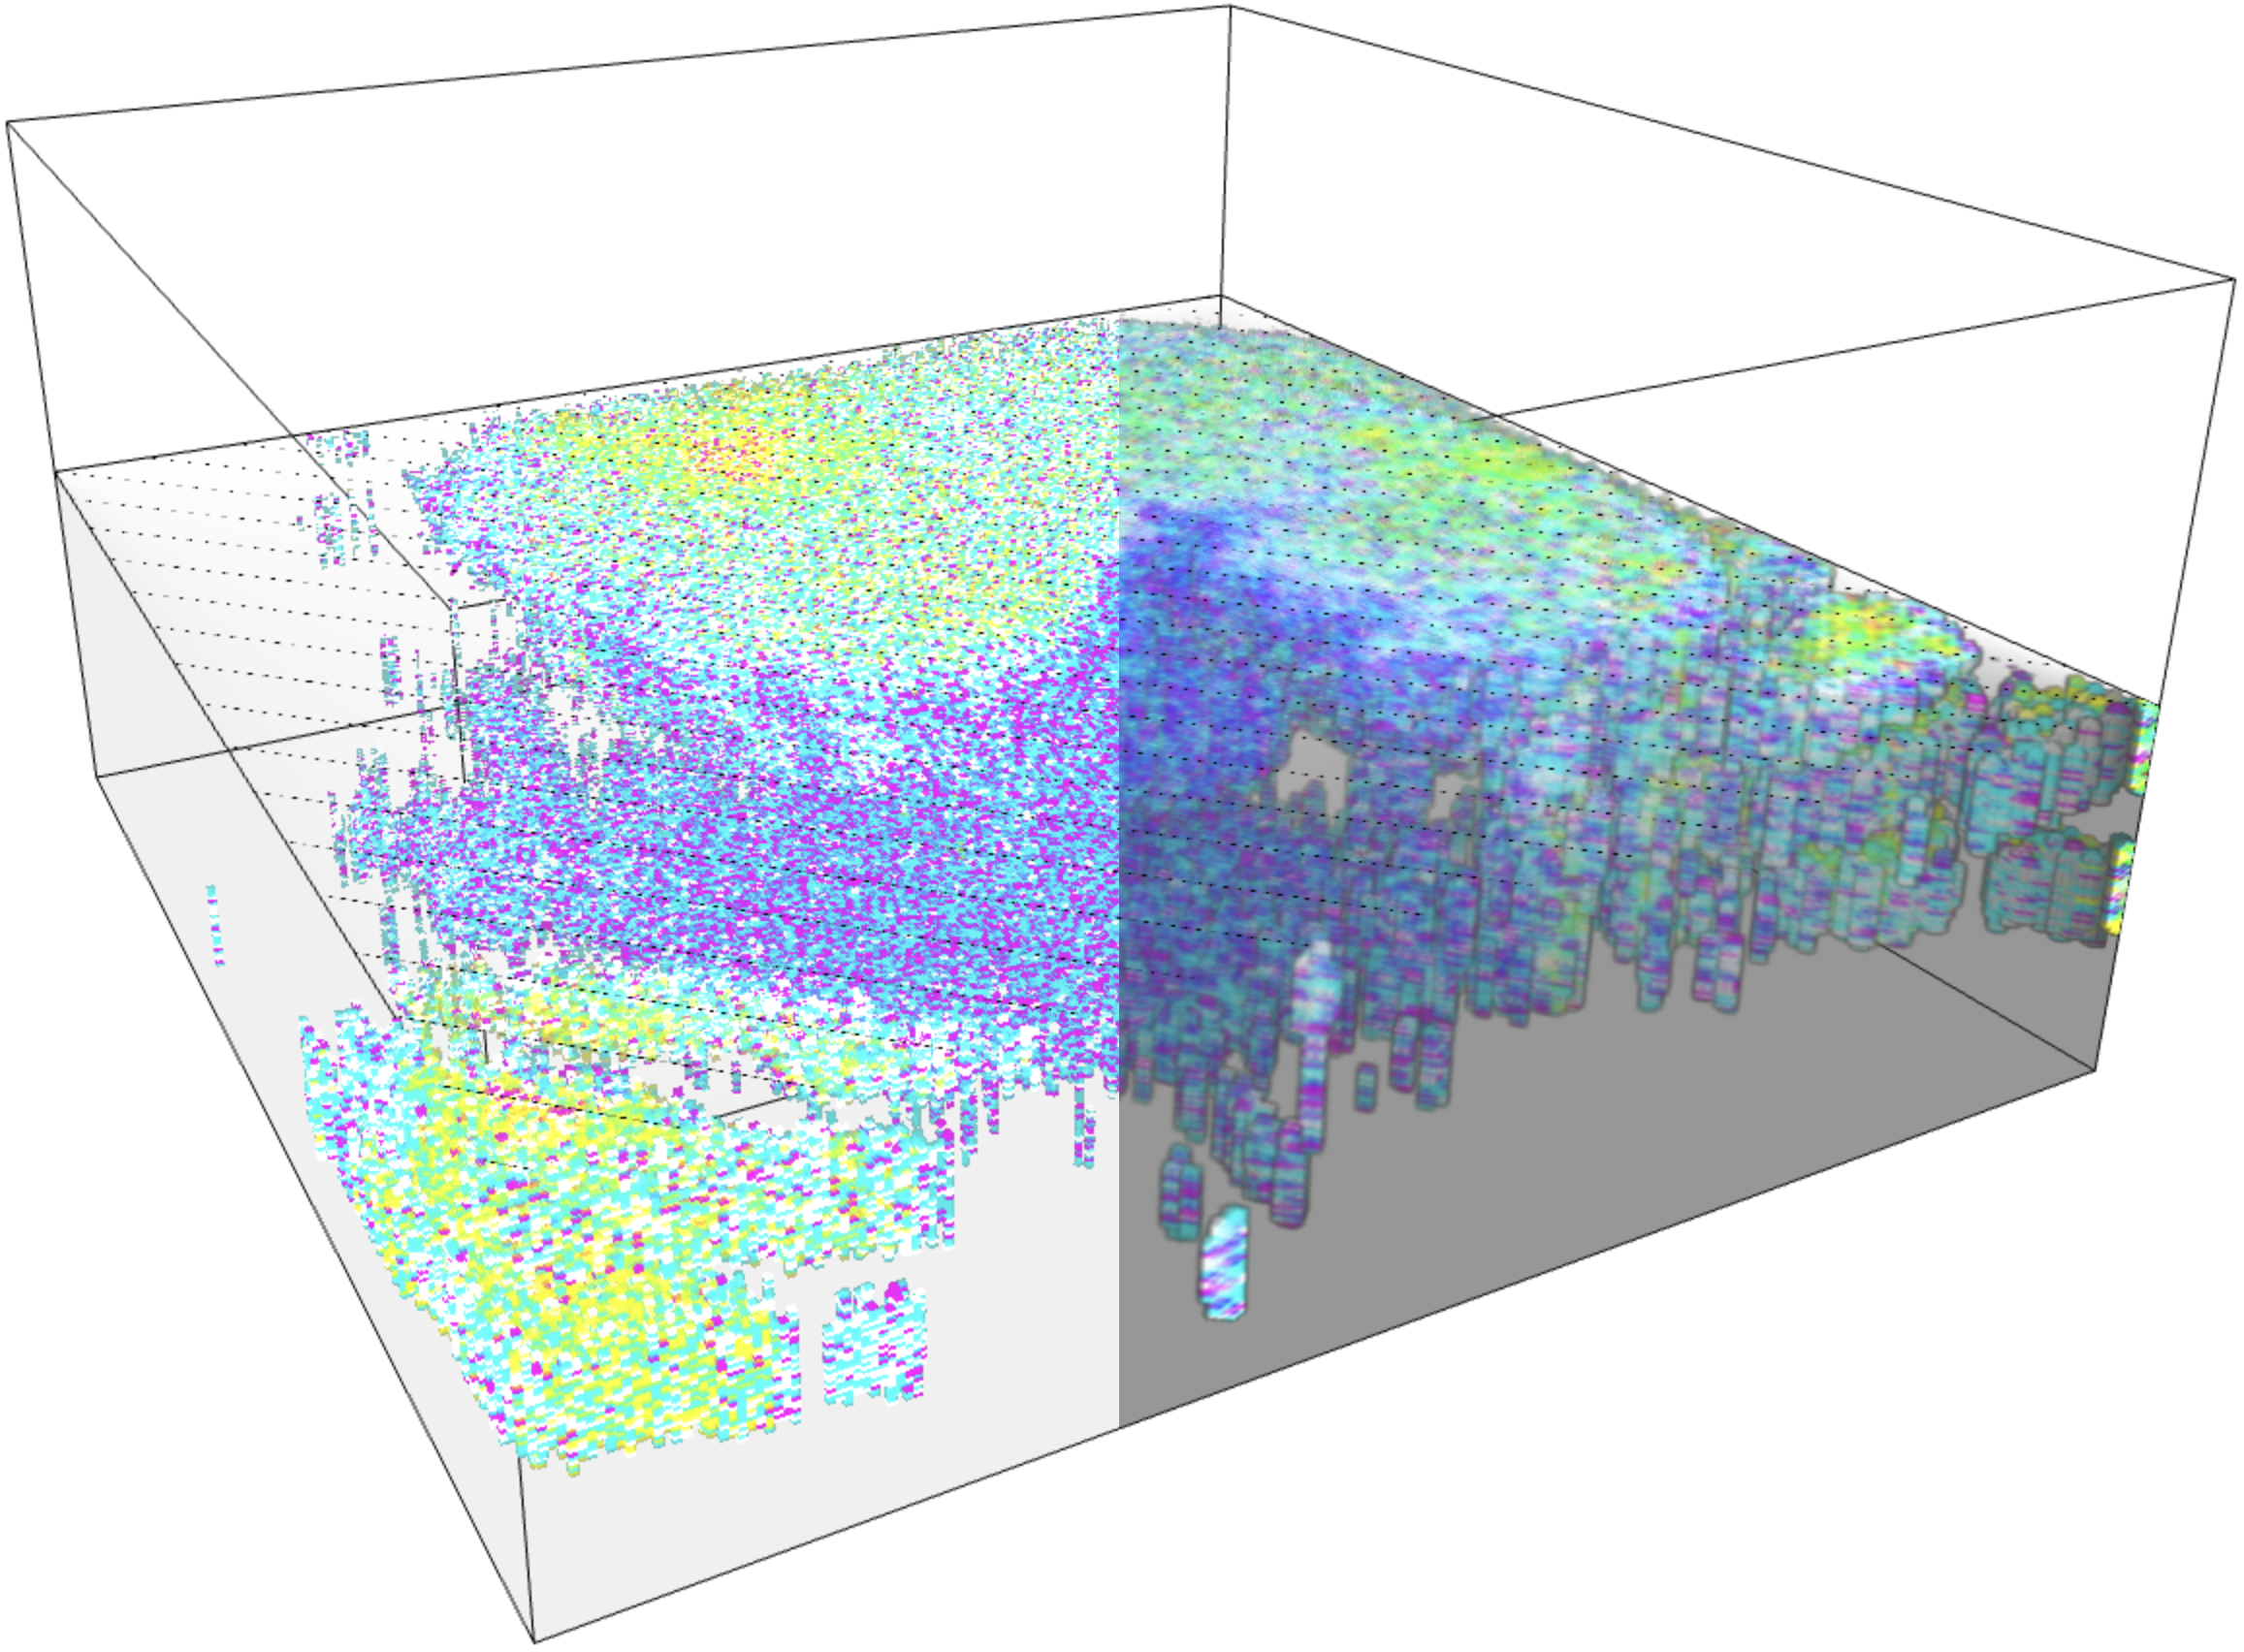
\includegraphics[width=\columnwidth]{images/preview-merged.png}

\vspace{.25in}

\begin{multicols}{2}

\section{Abstract}

3d printing has enabled the creation of otherwise impossible objects by providing the ability to define an object via a mesh and reproduce that mesh into a real, handheld object.

Most print technologies, however, are limited to this mesh format, and are unable to accurately (both aesthetically and meaningfully) recreate objects and representations of data that are not able to be reasonably ``crunched" into a mesh. This could be things like radar pictures of weather systems (as pictured in the title image), to things like fires or explosions that the computer graphics world would define with particle systems.

While solutions for printing from pointcloud data sources do exist, none provide the unrivaled freedom as being able to program exactly what material goes in each position like GrabCAD Voxel Print on Stratasys PolyJet systems enables.

\section{Introduction \& background}

This whitepaper covers the process of ingesting images and converting them to `slice' files ready for the Voxel Print system.

Among the wide collection of additive manufacturing methodologies is a technique called material-jetting, or (as referred to in the Stratasys portfolio) PolyJet. PolyJet systems work by depositing tiny dots of photopolymer resin, immediately exposing them, and continuing to further layers. 

\subsection{Limitations \& equipment}

The work covered by this publication was completed on a Stratasys J735 PolyJet 3d printer, and requires GrabCAD Print Pro in order to have access to the Voxel Print utility. 

This paper skips the data acquisition \& initial processing steps.

The final solution of this paper is an approximation of colors that is acceptable for most use cases. Outcomes will not have perfect color accuracy as the application of color calibration may not be perfect for all printer configurations, dithering \& half-toning algorithms, and environment. A more color-accurate approach is described in ``Color-Managed 3D-Printing with highly Translucent Printing Materials"\footnote{``Color-Managed 3D-Printing with highly Translucent Printing Materials, Can Ates Arikan, Alan Brunton, Tejas Madan Tanksale and Philipp Urban"}. For the purposes of everyday 3d printing, the approach described herein strikes an appropriate balance between appearance \& accuracy with the workload and upfront resources required.

\section{Objective/end-state}

The high-level objective of the utility this paper describes is an application that takes in an sRGB image and converts it into am image that is ready to provide to the PolyJet printer, where each pixel is an explicit material assignment.

\section{High-level overview}

The voxel printing pipeline can be described in 2 basic steps: the application of color correction and halftoning steps.

\subsection{Color Correction}
\vspace{1mm}

\noindent
\begin{tabular}{@{} c l @{}}

  % --- First image + text ---
  \begin{minipage}{0.25\linewidth}
    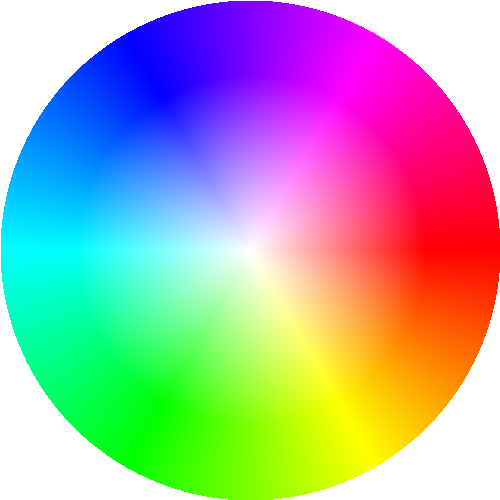
\includegraphics[width=\linewidth]{images/source-wheel.png}
  \end{minipage}
  &
  \begin{minipage}{0.7\linewidth}
    \textbf{(a) Source Data} To apply the color correction methods, the process starts with the generated color wheel PNG image. This image is in sRGB and sourced directly from a color wheel generator function.
  \end{minipage}
  \vspace{1mm}
  \\[0mm]
  \(\downarrow\)
  &
  \\[0mm]

  \begin{minipage}{0.25\linewidth}
    
\includegraphics[width=\linewidth]{images/color-converted.png}
  \end{minipage}
  &
  \begin{minipage}{0.7\linewidth}
    \textbf{(b) Color Corrected} Using ImageMagick, the workflow produces the color corrected image. As a default, the process should use the system's native sRGB profile as a source and the profile from the printer as the destination.
  \end{minipage}

\end{tabular}

\vspace{3mm}


Attempting to print accurate colors complicates the Voxel Print pipeline. While simply halftoning an sRGB (or other) image will lead to a print that has the same primary colors (especially powerful colors like purples and blues), weaker colors like yellows will be washed out and overpowered. Color correction can be applied to fix these ratios and force colors to be re-balanced. 

Stratasys has already done the spectrophotometry for their printers and common material combinations. These color profiles are stored in GrabCAD Print but can be extracted by saving a .print file. Using an unzip utility (or renaming file's extension from .print $\rightarrow$ .zip), the embedded files of a print project can be accessed, one of which will be a color correction profile (extension .icm or .icc).

That color profile extracted from the printer is what the workflow will apply to the images to strengthen the weak colors and to tame the stronger colors.

\subsection{Quantization \& halftoning}

\vspace{1mm}

\noindent
\begin{tabular}{@{} c l @{}}

  % --- First image + text ---
  \begin{minipage}{0.25\linewidth}
    
\includegraphics[width=\linewidth]{images/color-converted.png}
  \end{minipage}
  &
  \begin{minipage}{0.7\linewidth}
    \textbf{(a) Color Corrected} The input to the quantization and halftoning algorithm is a color-corrected image. 
  \end{minipage}
  \vspace{1mm}
  \\[0mm]
  \(\downarrow\)
  &
  \\[0mm]

  \begin{minipage}{0.25\linewidth}
    
\includegraphics[width=\linewidth]{images/layer_00.png}
  \end{minipage}
  &
  \begin{minipage}{0.7\linewidth}
    \textbf{(b) Quantized \& Halftoned slice} This stage will provides slice files that are reduced to the strict 6 colors. It converts from any human-friendly color images to specific voxel instruction slices.
  \end{minipage}

\end{tabular}

\vspace{3mm}

\subsubsection{Fully-saturated colors}

The color step involves a simple subtractive conversion from RGB to CMY for each pixel

\[
H(r,g,b) = 
\left\{
\begin{array}{l}
c = 1 - \frac{r}{255} \\[6pt]
m = 1 - \frac{g}{255} \\[6pt]
y = 1 - \frac{b}{255}
\end{array}
\right.
\]

Then, random decisions determine which pigment actually prints at that location. After converting the pixel from RGB to CMY, each of the cyan, magenta, and yellow values becomes the probability that the slice will command to print that resin. Instead of choosing among them proportionally, the algorithm runs three independent Bernoulli trials—one for C, one for M, one for Y. Each trial is a simulation of the question: ``Which resin should be at this voxel?" If its random draw falls below its probability, that resin becomes a candidate. If one or more resins pass their trials, one is randomly selected from that candidate set. If none pass, the process falls back to a luminance calculation. This workflow is a form of stochastic point-process halftoning, where every channel decision is made independently and locally.

Straight probability cannot be used (e.g., skipping the Bernoulli trials), because a color such as cmy(1, 0.6, 0.8) — a deep green — would always yield cyan; any random value in [0, 1] would fall below the cyan probability and no other channel would ever be selected.

As an example for how the color logic works, here is a trace for how to pipeline will process a color like Saint Louis University's Oriflamme Orange (\texttt{\#ED8B00}).

The process begins by converting Oriflamme Orange using the color correction profile (in this case, the `Stratasys\_J750\_Vivid\_CMY\_1mm.icm' from the printer). This results in a working color of \texttt{\#faa236} (\texttt{rgb(250, 162, 54)}).

\[
\vcenter{\hbox{\texttt{\#ED8B00}}}
\;\xrightarrow{}\;
\vcenter{\hbox{
\includegraphics[width=0.05\linewidth]{images/oriflamme-orange-uncorrected.png}}}
\;\xrightarrow{}\;
\vcenter{\hbox{
\includegraphics[width=0.05\linewidth]{images/oriflamme-orange-corrected.png}}}
\;\xrightarrow{}\;
\vcenter{\hbox{\texttt{cmy(0.019,\,0.364,\,0.788)}}}
\]

The first step is to compute the cyan, magenta, and yellow values from the rgb. This method ($H$) is outlined above. Those then become the sources for the independent Bernoulli trials. Using this method, run one independent trial per channel:

\begin{itemize}
    \item C trial: probability = 0.019 \\
   	$\rightarrow$ fires if rand() $<$ 0.019 ($\approx$1.9\% chance)
 
    \item M trial: probability = 0.364 \\
   	$\rightarrow$ fires if rand() $<$ 0.364 ($\approx$36.4\% chance)
   	
    \item Y trial: probability = 0.788 \\
   	$\rightarrow$ fires if rand() $<$ 0.788 ($\approx$78.8\% chance)
\end{itemize}

\noindent
Once trials have been defined, they get tested:

\begin{itemize}
	\item If C trial succeeds, add Cyan to a candidates list
	\item If M trial succeeds, add Magenta to candidates
	\item If Y trial succeeds, add Yellow to candidates.	
\end{itemize}

\noindent
This results in the following outcome cases:

\begin{itemize}
	\item Case 1 (most likely):
	Only Y and/or M fire, leaving the list of possible candidates:
	\begin{itemize}
		\item{[``yellow"]}
		\item{[``magenta"]}
		\item{[``yellow", ``magenta"]}
	\end{itemize}
	\item Case 2 (less likely):
	Cyan fires, so it could also show up in the candidate set.
	\item Case 3 (less likely)
	None of the 3 possible variables fire and the process fall back to the luminance flow.
\end{itemize}

\noindent
After the candidate list is computed, the number of passing cases is given by the length of that list. A uniformly random selection is then made from the candidates for each voxel, and the selected entry determines the resin deposited at that location.

Given these flows and simulations, the expected distribution is roughly 49\% of the candidate lists to be solely yellow, 28\% of the candidate lists to be yellow or magenta, 13\% of lists to be solely magenta, less than 2\% combined of all other possible combinations\footnote{["yellow", "cyan"], ["magenta", "cyan"], ["cyan"], ["yellow","magenta","cyan"]}, and approximately 0.13\% to contain no values at all, in which case the process falls back to the luminance branch.

This candidate behavior produces an expected distribution of approximately 63.8\% of pixels to be yellow, 21.8\% of pixels to be magenta, 0.09\% of pixels to be cyan, and about 13.2\% to be white or `black'.

The final generated slice looks something like this (500px wide by 100px tall):

\

\noindent

\includegraphics[width=\linewidth]{images/orfi-layer_00.png}

A pixel count of the image confirms that the process performed as intended:

\

\noindent
\begin{tabularx}{\columnwidth}{X r r}
\textbf{Color} & \textbf{Pixel Count} & \textbf{Percent} \\ \hline
cyan    & 511   & 1.0220\% \\
magenta & 10896 & 21.7920\% \\
yellow  & 31946 & 63.8920\% \\
white   & 6647  & 13.2940\% \\
\end{tabularx}

\subsubsection{Transparency}

Transparency is decided the same as colors, where a 50\% transparent pixel will have a 50\% chance of a transparent drop of resin, and a 50\% chance of progressing into the normal color halftoning pipeline.

\subsubsection{Luminance}

Starting with the RGB values of a color-corrected pixel, the Rec.709 luminance formula is applied:


\[
Y = 0.212\left(\tfrac{R}{255}\right)
  + 0.715\left(\tfrac{G}{255}\right)
  + 0.072\left(\tfrac{B}{255}\right)
\]

This provides the perceived brightness of the pixel. If no other pixels ``hit" in the fully-saturated color pass, This luminance value $Y$ is used to determine whether to put a white pixel down or to approximate black.

Because the J735 full-color configuration typically does not include black resin, black is approximated using a mixture of cyan, magenta, and yellow resins. Passing true black (\#000000) into the color-correction pipeline provides the thresholds used for this approximation:

\[
\begin{array}{l}
c = 1 - \frac{0}{255} = 1 \\[6pt]
m = 1 - \frac{66}{255} = 0.741 \\[6pt]
y = 1 - \frac{124}{255} = 0.486
\end{array}
\]

\noindent
Applying the independent Bernoulli-trials algorithm described in the fully-saturated colors section and then scaling the resulting probabilities upward to ensure that each pixel is assigned cyan, magenta, or yellow (with white dots excluded in pure-black regions) produces an overall distribution of approximately 31\% cyan, 31\% magenta, 12\% yellow, with the remaining pixels going to the transparent branch.

This approach to black will provide an accurate approximation for black pixels in source data images. For a true perceptual "forced" black, these percentages would be dragged up to force each pixel to be either c, m, or y. These re-scaled values would be:

\[
\begin{aligned}
s &= c + m + y =1 + 0.741 + 0.486 &= 2.227 \\
c &= {c}/{s}   = {1}/{2.227} &= 0.449 \\
m &= {m}/{s}   = {0.741}/{2.227} &= 0.333\\
y &= {y}/{s}   = {0.486}/{2.227} &= 0.218 \\
\end{aligned}
\]

Grayscale uses the same independent Bernoulli trials, but only between white and the now-defined black approximation.

\subsubsection{Stochastic halftoning vs ordered dithering}

Traditional ordered dithering algorithms (such as Bayer matrices or Floyd-Steinberg) produce excellent results for 2D screen graphics, but they are not well-suited for voxel-level PolyJet printing. Ordered dithering enforces a spatial pattern that repeats across the image, causing structured artifacts (grids, diagonals, clusters, and periodic textures). These artifacts are amplified by the repetition of slices in PolyJet prints. The deterministic nature of these algorithms makes it impossible to randomize voxel color placement.

Stochastic halftoning avoids this entirely. Each voxel decision is made independently using local probabilities, which produces a noise-like distribution of materials with no repeating artifacts. By nature of it being stochastic, this approach is non-deterministic. This helps prevent a ``speckled" appearance in the final print.

In non-technical language, despite the fact that each slice's source data image might be identical, the actual slices need to be different. The arrangement of color ratios need to be randomized. 

\section{Post-processing files}

Due to the printer's non-square pixel density ratio, the images need to be scaled by 2x in the horizontal axis (since the printer is 300 dpi x 600 dpi). Depending on how the color correction and halftoning algorithms work, it may also be necessary to re-crop layers before printing.

\section{Conclusion}

The workflow described in this paper demonstrates a practical and reproducible approach to translating 2D raster imagery into 3D voxel-based data suitable for Stratasys PolyJet Voxel Print systems. By combining standardized ICC-based color correction and stochastic halftoning, this approach can achieve prints that preserve the visual fidelity and relative luminance balance of the source image while conforming to the material and process limitations of PolyJet printing.

This process bridges the gap between digital imagery and volumetric material assignment, unlocking new possibilities for printing scientific visualizations, artistic pieces, and complex multi-material designs that cannot be represented by traditional mesh models. While this approach is not perfectly color-managed, it provides a strong foundation for experimental workflows that prioritize creative control and reproducibility. 

\end{multicols}

\end{document}
